\documentclass[11pt]{article}
\usepackage{MyTemplate}
\begin{document}
\newcommand{\multispec}{چندطیفی}
\newcommand{\hyperspec}{ابرطیفی}
\newcommand{\isomap}{آیزومپ}
\newcommand{\lle}{تعبیه‌ی موضعی خطی }
\newcommand{\LTSA}{تنظیم موضعی صفحه‌ی مماس}
\newcommand{\LapEig}{نگاشت ویژه‌ی لاپلاسینی}
\newcommand{\landmarkisomap}{\lr{لندمارک-آیزومپ}}
\newcommand{\landmark}{نماینده}
%\newcommand{\endmember}{جزء خالص}
\newcommand{\inductive}{استنتاجی}
\newcommand{\transductive}{ورارسانی}
\newcommand{\multidimscale}{تغییر مقیاس چند بعدی}
\newcommand{\knowledgetransfer}{انتقال دانش}
\newcommand{\likelihood}{شباهت}
\newcommand{\overfitting}{تطبیق بیش از حد}
\newcommand{\curseOfDim}{مشکل بعد}
\newcommand{\ememb}{عنصر نهایی}
\newcommand{\generative}{مولد}
\newcommand{\discriminative}{تمایزدهنده}
\newcommand{\kernel}{هسته}
\newcommand{\oAo}{دسته‌بندی یک با یک}
\newcommand{\oAa}{دسته‌بندی یک با همه}
\newcommand{\EM}{\lr{EM}}
\newcommand{\SVM}{ماشین بردار پشتیبان}
\newcommand{\transductiveSVM}{\SVM{} \transductive{}}
\newcommand{\kmeans}{\lr{k}-میانگین}
\newcommand{\urbundetection}{تشخیص مناطق شهری}
\newcommand{\LGC}{سازگاری محلی و عمومی}
\newcommand{\regularization}{منظم‌سازی}
\newcommand{\tikhonov}{تیخونوف}
\newcommand{\PCA}{تحلیل مولفه‌ی اصلی}
\newcommand{\residualvar}{واریانس باقیمانده}
\newcommand{\gaussianprocess}{فرایند گاوسی}
\newcommand{\lossfunction}{تابع ضرر}
\newcommand{\RKHS}{فضای هیلبرت بازتولید هسته}
\newcommand{\hinge}{لولا}
\newcommand{\noisy}{نویزی}
\newcommand{\RBF}{\lr{RBF}}
\newcommand{\difL}{انتشار لاپلاسین}
\newcommand{\LapSVM}{ماشین بردار پشتیبان لاپلاسینی}
\newcommand{\embedding}{بازنشانی}
\newcommand{\SVDD}{تشخیص دامنه‌ی بردار پشتیبان}
\thispagestyle{empty}
\settextfont[Scale=1.2]{B Nazanin}
\begin{center}

\includegraphics{logo}
\vskip 1cm
{\bf
دانشگاه صنعتی شریف\\ دانشکده مهندسی کامپیوتر\\ سمینار کارشناسی ارشد گرایش هوش مصنوعی\\
\vskip 1cm
عنوان:\\
بر چسب گذاری داده با استفاده از يادگيری نيمه نظارتی مبتنی بر منيفلد در داده‌های \multispec{} سنجش از راه دور\\
\lr{Data Labelling Using Manifold-Based Semi-Supervised Learning in Multispectral Remote Sensing}
\vskip 1cm
نگارش:\\
احمد خواجه‌نژاد\\
89210841\\
\vskip 1cm
استاد راهنما:\\
دکتر محمدعلی صفری - دکتر حمیدرضا ربیعی\\
\vskip 1cm
استاد ممتحن داخلی:\\
دکتر مهدی جلیلی\\

\vskip 3.5cm

}
دی ۹۰
\newpage
\end{center}



\settextfont{B Nazanin}

{\bf {چکيده: }}
مساله‌ی تشخیص برچسب هر نقطه از یک تصویر سنجش از دور که در ابتدا فقط برچسب برخی از نقاط آن را می‌دانیم، با نام دسته‌بندی تصاویر سنجش از دور شناخته شده است. به دلیل ویژگی‌های این مساله، مثل تعداد زیاد داده‌ها و تعداد کم داده‌های برچسب‌دار، روش‌های یادگیری نیمه‌نظارتی در آن کاربرد زیادی دارند. به طور کلی، روش‌های نیمه‌نظارتی استفاده شده در این مساله را می‌توان به سه دسته‌ی روش‌های \generative{}، روش‌های مبتنی بر جداسازی در ناحیه‌ی کم تراکم و روش‌های مبتنی بر گراف (منیفلد) تقسیم کرد. در این گزارش، ابتدا به تعریف مساله و ویژگی‌های خاص آن پرداخته، سپس در مورد سه دسته روش مذکور توضیحاتی ارائه کرده و با تمرکز بر روش‌های مبتنی بر گراف، به مقایسه‌ی تئوری و عملی این روش‌ها می‌پردازیم.

{\bf  { واژه‌های کلیدی: }}
 سنجش از دور، یادگیری نیمه‌نظارتی، منیفلد، \multispec{}، \hyperspec{}


\setlength{\parindent}{0.25in} %The indent of the paragraph first line

\section{مقدمه}\label{intro}

به طور کلی سنجش از دور، به معنی کسب اطلاعات از طریق تحلیل داده‌های به دست آمده از تصاویر و امواج برداشت شده از راه دور از شیء، مکان یا پدیده‌ای می‌باشد. در این پژوهش، هدف تحلیل داده‌های به دست آمده از عکس‌های هوایی یا ماهواره‌ای است. در عکس‌های \lr{RGB} معمولی، فقط میزان نور بازتاب شده در محدوده‌ی طول موج‌های قابل دید، در سه بازه‌ی مربوط به رنگ های قرمز،
% ( 620-740 نانومتر) 
سبز
% (520-570 نانومتر)
و آبی
% (440-490 نانومتر)
 ذخیره شده است. اما در عکس‌های مورد مطالعه‌ی ما میزان نور بازتاب شده از هر نقطه در باندهای طیفی (یعنی همان بازه‌های طول موج) مرئی و غیر مرئی مختلف ذخیره شده است، بنابراین اگر مثلا اطلاعات مربوط به 8 بازه‌ی فرکانسی ذخیره شده باشد، هر پیکسل به صورت یک بردار به طول 8 از اعداد می‌باشد. به همین دلیل این عکس‌ها را چندطیفی\LTRfootnote{\lr{multispectral}}
می‌گویند‌. به بیان دیگر  می‌توان این عکس‌ها را به صورت تعدادی عکس (سیاه و سفید) از یک منطقه در نظر گرفت که هر عکس مربوط به یک باند طیفی است. 
معمولا اگر باندهای طیفی عریض بوده و تعداد آن‌ها کم (در حدود 10 باند) باشد، تصویر را چندطیفی گویند، اما اگر باندها باریک بوده و تعداد آن‌ها زیاد باشد، تصویر را \hyperspec{}\LTRfootnote{\lr{hyper-spectral}}  می‌گویند. زمانی که کاربرد مورد نظر ما به صورتی است که نیاز به بررسی تغییرات کوچک در باندهای باریک دارد، استفاده از تصاویر \hyperspec{} لازم می‌شود. تمرکز ما هم در این پژوهش بر تحلیل داده‌های \hyperspec{} است.


در تحلیل عکس‌های \hyperspec{}، چند هدف وجود دارد که مساله‌ی اصلی مورد بررسی ما در این پروژه، دسته‌بندی\LTRfootnote{\lr{classification}}
می‌باشد. این مساله را برچسب‌گذاری\LTRfootnote{\lr{labeling}} یا نوعی قطعه‌بندی\LTRfootnote{\lr{segmentation}} هم می‌توان نامید. در این مساله هدف این است که از روی تصاویر موجود، برچسب مربوط به هر نقطه (پیکسل) را تشخیص دهیم. بسته به کاربردهای مختلف، این برچسب می‌تواند بافت زمین، پوشش گیاهی، عمق آب یا موارد دیگر باشد. البته در مواردی مثل تشخیص عمق آب، مجموعه‌ی مقادیر مجاز به عنوان برچسب یک پیکسل، یک بازه‌ی پیوسته‌ می‌باشد. بنابراین در این حالت با یک مساله از نوع رگرسیون مواجه هستیم، نه دسته‌بندی. در دسته‌بندی، هر نقطه برچسبی دارد که یکی از چند مقدار مشخص را می‌تواند داشته باشد.

به عنوان داده‌های ورودی مساله، ما مقادیر طیفی مربوط به همه‌ی پیسکل‌ها و برچسب بعضی از پیکسل‌ها را می‌دانیم، و هدف این است که برچسب نقاط بدون برچسب را پیش‌بینی کنیم. البته در اغلب کاربردهای دسته‌بندی، می‌توانیم مساله را به این صورت بیان کنیم که تصویر به نواحی‌ای تقسیم می‌شود و نقاط هر ناحیه، برچسب یکسانی دارند (نقاط دو ناحیه‌ی جدا از هم می‌توانند برچسب یکسانی داشته باشند) و ما می‌خواهیم با داشتن نمایش طیفی تمام نقاط و برچسب برخی از آن‌ها، تمام نواحی موجود و برچسب مربوط به هر ناحیه را پیدا کنیم.


زیاد بودن تعداد ابعاد فضای داده‌ها در مسائل یادگیری ماشین، پیچیدگی مسائل را زیاد می‌کند. این مفهوم شناخته شده‌ای است که از آن با نام \curseOfDim{}\LTRfootnote{\lr{curse of dimensionality}}
یاد می‌شود. بنابراین پیدا کردن تعداد کمی پایه‌ی مناسب که بتوان داده‌ها را در فضای ساخته شده از آن‌ها بیان کرد، به طوری که پراکندگی داده‌ها حفظ شود، از اهمیت زیادی برخوردار است. این کار را استخراج ویژگی\LTRfootnote{\lr{feature extraction}} می‌نامند. در مسائل مربوط به سنجش از دور، چون با داده‌های \hyperspec{} سر و کار داریم، مساله‌ی استخراج ویژگی اهمیت زیادی پیدا می‌کند. بنابراین مساله‌ی استخراج ویژگی نیز مورد توجه ما خواهد بود.


در سنجش از دور، مسائل دیگری نیز وجود دارد که البته ما به آن‌ها نخواهیم پرداخت، اما با اخذ از 
\cite{ML_in_RS}
بعضی از آن‌ها را بیان می‌کنیم. مثلا در مساله‌ی تشخیص تغییر\LTRfootnote{\lr{change detection}}،
 عکس‌هایی از یک منطقه در زمان‌های متفاوت در دست داریم و هدف این است که تغییرات نواحی را در طول زمان تشخیص دهیم. برای مثال در تشخیص گسترش مناطق شهری یا تغییر نوع پوشش گیاهی یا تغییر نواحی در اثر زلزله با این مساله مواجه هستیم.
 
 
از دیگر مسائل موجود در این زمینه خوشه‌بندی\LTRfootnote{\lr{clustering}}
و تجسم داده\LTRfootnote{\lr{data visualizasion}}
است. خوشه‌بندی ممکن است به صورت کاربرد مستقل یا پیش‌پردازشی برای کاربردهای دیگر مثل دسته‌بندی انجام شود. همچنین تجسم داده‌ها می‌تواند برای تحلیل بصری داده‌ها مفید باشد.

در یک عکس، هر  پیکسل‌ ترکیبی از الگوی بازتابی مواد تشکیل‌دهنده‌ی آن است. در مساله‌ی تجزیه‌ی سیگنالی\LTRfootnote{\lr{signal unmixing}}
هدف آن است که پیکسل‌های خالصی را به عنوان پایه پیدا کنند که بتوانند نمایش طیفی هر پیکسل را با استفاده از ترکیبی خطی از آن‌ها نمایش دهند. این پیکسل‌های پایه را به اصطلاح 
\ememb{}\LTRfootnote{\lr{endmember}}
می‌گویند.

همچنین در مسائلی که مدلی برای بازتاب طیفی نقاط فرض کرده‌اند و می‌خواهند پارامترهای مدل را پیدا کنند، مساله‌ی رگرسیون و معکوس‌یابی مدل\LTRfootnote{\lr{model inversion}}
مطرح می‌شود.


همان‌طور که گفته شد، تاکید ما در این پروژه بر مساله‌ی دسته‌بندی برای تصاویر \hyperspec{} است، که در نتیجه با استخراج ویژگی هم درگیر خواهیم بود. رویکرد ما به این مساله با مفروضات و رویکردهای خاصی است که در ادامه به آن‌ها اشاره می‌شود.

\section[ویژگی‌های مساله]{
ویژگی‌های مساله
}
مساله‌ی مورد بررسی، در نگاه اول یک مساله‌ی دسته‌بندی ساده می‌باشد، اما در  واقع به دلیل ویژگی‌هایی که دارد، مساله‌ای خاص می‌باشد. این ویژگی‌‌ها بدین صورت می‌باشند:
\begin{itemize}
\item {زیاد بودن تعداد داده‌ها:}
چون در این مساله، هدف برچسب گذاری پیکسل‌های یک تصویر می‌باشد، معمولا با تعداد زیادی داده مواجه می‌باشیم. زیاد بودن تعداد داده‌ها، باعث افزایش بیش از حد زمان اجرا و حافظه‌ی مورد استفاده در بسیاری از الگوریتم‌ها می‌شود. به همین دلیل، یکی از چالش‌های مساله، و در نتیجه یک زمینه‌ی تلاش پژوهشگران در این مساله، ارائه‌ی روش‌های تقریبی برای الگورتم‌های مختلف، با زمان اجرا و حافظه‌ی کمتر می‌باشد.
\item {کم بودن تعداد داده‌های برچسب‌دار آموزش:}
در یک کاربرد واقعی، برچسب داده‌هایی که قرار است در فاز آموزش استفاده شوند، یا به وسیله‌ی بررسی عکس توسط متخصص و تعیین برچسب برخی نقاط تعیین می‌شود، یا از طریق بررسی نقاط واقعی در مکان (مثلا در کاربرد تشخیص منابع زیرزمینی) یا به صورت ترکیب این دو روش. در هر صورت، تعیین برچسب نقاط کاری سخت و هزینه‌بر است. بنابراین به دنبال یافتن روشی هستیم که بتواند با استفاده از تعداد کمی داده‌ی برچسب‌دار دسته بندی را به خوبی انجام دهد.
\item {بعد بالای داده‌ها:}
زیاد بودن تعداد ابعاد داده‌ها هم دقت یادگیری را کاهش می‌دهد، و هم برای ذخیره و ارسال داده‌ها از ماهواره به زمین ایجاد مشکل میکند. به همین دلیل برخی تلاش‌ها صرفا در جهت کاهش بعد داده‌ها به نحوی که جدایی پذیری آن‌ها حفظ شود، می‌باشد.
%البته در مواردی هم از این تعداد زیاد بعد، به عنوان ابزاری برای ساختن دسته‌بندهای مختلف و ترکیب آن‌ها با یکدیگر استفاده شده است.
\item {وابستگی مکانی نقاط به یکدیگر:}
در ساده‌ترین حالت، می‌توان بردار ویژگی مربوط به هر پیکسل را همان نمایش طیفی آن (مقدار نور بازتاب شده از آن نقطه در هر بازه‌ی طول موج) در نظر گرفت. اما چون نقاط تصویر قابل تقسیم به نواحی‌ای می‌باشد که در هر ناحیه برچسب تمام نقاط یکسان است، پس در واقع احتمال متفاوت بودن برچسب دو نقطه که فاصله‌ی مکانی کمی دارند، زیاد نیست. از این ویژگی می‌توان در یادگیری استفاده کرد. از ایده‌های اصلی که برای استفاده از این ویژگی مطرح شده است، می‌توان ناحیه‌بندی\LTRfootnote{\lr{segmentation}} و میانگین‌گیری را نام برد. در ناحیه‌بندی، ابتدا در یک فاز غیرنظارتی\LTRfootnote{\lr{unsupervised}}، تصویر به نواحی مختلفی افراز می‌شود، سپس از هر ناحیه نمایندگانی انتخاب می‌شوند و یادگیری فقط با توجه به آن‌ها انجام می‌شود.

روش میانگین‌گیری به این صورت است که بردار ویژگی مربوط به هر پیکسل، از ترکیب نمایش طیفی همان پیکسل، با میانگین نمایش طیفی نقاط در یک همسایگی آن نقطه ساخته می‌شود. در روش‌های یادگیری مبتنی بر \kernel{}، می‌توان یک \kernel{} مبتنی بر نمایش طیفی نقاط، و یک \kernel{} مبتنی بر میانگین نمایش طیفی در همسایگی هر نقطه تعریف کرده و این دو \kernel{} را به روش‌های مختلف موجود با یکدیگر ترکیب کرد تا \kernel{} جدیدی به دست بیاید.

نکته‌ی شایان توجه دیگر این که با توجه دو روشی که برای برچسب‌گذاری نقاط ذکر شد، این طور به نظر می‌رسد که در کاربرد واقعی، داده‌های برچسب‌دار ما در فاز آموزش، تعدادی پیکسل پراکنده نیستند، بلکه طبعا به این صورت است که فرد متخصص، تعدادی ناحیه - که هر ناحیه شامل تعدادی پیکسل است - را مشخص کرده و برچسب مربوط به هر ناحیه را می‌گوید.
\item {چندکلاسه بودن مساله:}
بسیاری از روش‌های دسته بندی، برای مسائل دو کلاسه ارائه شده‌اند. بنابراین برای تعمیم به حالت چندکلاسه، مجبور به استفاده از روش‌هایی مثل \oAo{}\LTRfootnote{\lr{one against one}} یا \oAa{} \LTRfootnote{\lr{one against all}} می‌باشیم. البته در روش‌های نیمه‌نظارتی، چون از داده‌های بدون برچسب هم در یادگیری استفاده می‌شود، استفاده از روش \oAo{} چندان درست نیست، زیرا در این صورت، برای تمایز بین دو کلاس، از داده‌های بدون برچسب مربوط به سایر کلاس‌ها هم به عنوان داده‌های مربوط به این دو کلاس استفاده خواهیم کرد.
\end{itemize}

\section {استخراج ویژگی}
همان‌طور که در بخش \ref{intro} گفته شد، زیاد بودن تعداد ابعاد، دقت دسته‌بندی را کاهش می‌دهد. همچنین این مساله، در حجم داده‌هایی که باید ذخیره و احتمالا به مقصدی ارسال شوند هم ایجاد مشکل می‌کند. یعنی اگر روش خوبی برای کاهش بعد داده‌ها وجود داشته باشد، ‌می‌توان داده‌ها را پس از عکس‌برداری ابتدا کاهش بعد داد، و سپس از ماهواره به زمین ارسال کرد.

بنابراین برای سنجش میزان کارایی یک روش کاهش بعد، دو معیار وجود دارد، یکی تعداد ابعاد لازم برای ذخیره‌ی مقدار مورد نظر از انرژی داده‌ها، و دیگری تفکیک‌پذیری داده‌ها پس از کاهش بعد. معیار اول در روش‌هایی مثل \PCA{}\LTRfootnote{\lr{Principal Component Analysis}} و \isomap{}\LTRfootnote{\lr{Isomap}}، \residualvar{}\LTRfootnote{\lr{residual variance}}  است که نسبت واریانس نقاط در فضای جدید به واریانس آن‌ها در فضای اولیه (نسبت مجموع مقادیر ویژه‌ی مربوط به ابعاد مورد استفاده، به مجموع تمام مقادیر ویژه) می‌باشد.

اما تفکیک‌پذیری داده‌ها معمولا با سنجش دقت یک دسته‌بند ساده، مثلا دسته‌بند مبتنی بر $k$-\,نزدیک‌ترین همسایه، روی داده‌های کاهش بعد داده شده به روش‌های مختلف مقایسه می‌شود.

در \cite{Bachmann_exploiting} بر اساس این دو معیار نشان داده شده است که \isomap{} روش خوبی برای کاهش بعد داده‌های منیفلدی می‌باشد، و در مقالات دیگر از این مطلب به عنوان شاهدی برای این که داده‌های سنجش از دور، بر روی منیفلدی با تعداد ابعاد کم قرار دارند استفاده شده است. نویسندگان این مقاله، در مقالات بعدی در جهت بهبود زمان اجرا و حافظه‌ی مورد نیاز روش \isomap{} تلاش کرده‌اند، و نهایتا در \cite{Bachmann_improved}، روشی تخمینی برای \isomap{} ارائه کرده‌اند که زمان اجرای آن از مرتبه‌ی
 $O(n\lg^2n)$
و حافظه‌ی مورد نیاز آن از مرتبه‌ی
$O(n\lg{n})$
می باشد 
($n$ تعداد داده‌ها، یعنی همان تعداد پیکسل‌ها است).

از دیگر روش‌های معروف کاهش بعد مبتنی بر منیفلد، می‌توان  \lle{}\LTRfootnote{\lr{Locally Linear Embedding}}، \LTSA{}\LTRfootnote{\lr{Local Tangent Space Allignment}} و \LapEig{}\LTRfootnote{\lr{Laplacian Eigenmaps}} را نام برد. این روش‌ها خواص موضعی منیفلد را حفظ می‌کنند، یعنی سعی می‌کنند موقعیت نقاط نزدیک به یکدیگر در فضای اولیه، در فضای دوم نیز حفظ شود. این روش‌ها نیز در مقالات مختلفی مثل \cite{LLE1,LTS_1,LTS_2,Crawford_LML} بررسی شده‌اند.

ما در این پژوهش بر روش‌های کاهش بعد تمرکز نخواهیم کرد، زیرا هدف نهایی ما به دست آوردن دقت کافی در دسته‌بندی داده‌هاست. در ضمن با استفاده از روش‌های مبتنی بر \kernel{}، با اتخاذ \kernel{} مناسب می‌توان از افزایش خطا به دلیل تعداد زیاد ابعاد جلوگیری کرد. در مورد زمان اجرا و حافظه‌ی مورد نیاز هم، در اکثر روش‌های دسته‌بندی، تعداد زیاد داده‌ها عامل اصلی زیاد بودن زمان و حافظه‌ی مورد نیاز می‌باشد، نه تعداد ابعاد زیاد داده‌ها. نهایتا در صورتی که در روش خود نیاز به استفاده از کاهش بعد داشتیم، می‌توانیم از روش‌هایی که تا کنون مطرح شده‌اند استفاده کنیم. 


\section{
یادگیری نیمه‌نظارتی
}
در یادگیری نظارتی\LTRfootnote{\lr{supervised learning}}
آموزش به کمک داده‌هایی انجام می‌شود که برچسب تمام آن‌ها مشخص است. به عبارت دیگر در فاز آموزش تلاش می‌شود تا به کمک داده‌های برچسب‌دار و توزیع آن‌ها، ساختاری پیدا شود که بر اساس آن بتوانیم در فاز تست برچسب داده‌های تست را تعیین کنیم. اما در یادگیری نیمه‌نظارتی \LTRfootnote{\lr{semi-supervised learning}}
در فاز آموزش، علاوه بر داده‌های برچسب‌دار، تعدادی داده‌ی بدون برچسب هم در اختیار داریم که در تشخیص نحوه‌ی پراکندگی نقاط می‌توانیم از آن‌ها کمک بگیریم. به عنوان مثالی ساده فرض کنید برای دسته‌بندی داده‌های نشان داده شده در شکل \ref{fig:SSL} به دو دسته‌ی آبی و قرمز، بخواهیم مرزی پیدا کنیم که بر اساس آن نقاط صفحه را به دو دسته نسبت دهیم. اگر بخواهیم فقط از اطلاعات نقاط برچسب‌دار استفاده کنیم، احتمالا مرز را شبیه آن‌چه در شکل سمت چپ نشان داده شده است تعیین می‌کنیم. اما اگر  داده‌های بدون برچسب را هم در اختیار داشته باشم، مرزی که انتخاب می‌کنیم، چیزی شبیه به شکل سمت راست خواهد بود.		
\begin{figure}[h!]
  \begin{center}
    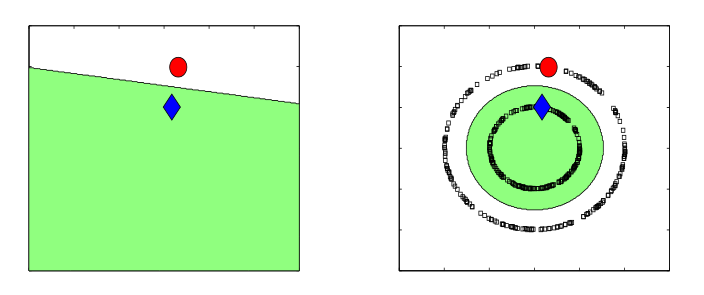
\includegraphics[width=0.7\textwidth]{images/semisupervised_learning.png}
    \caption{استفاده از داده‌های بدون برچسب در یادگیری \cite{Belkin_semisupervised}}
    \label{fig:SSL}
  \end{center}
\end{figure}

استفاده از یادگیری نیمه‌نظارتی، مخصوصا در مساله‌هایی مثل مساله‌ی ما که در آن‌ها برچسب‌گذاری دستی داده‌ها کار آسانی نیست و بنابراین تعداد داده‌های برچسب‌دار موجود کم است، همچنین تعداد زیادی داده‌ی بدون برچسب در اختیار داریم، بسیار مفید می‌باشد.

در یادگیری نیمه‌نظارتی، ممکن است هدف نهایی، برچسب‌گذاری همان داده‌های بدون برچسبی باشد که در فاز آموزش در اختیار داشتیم. این نوع یادگیری را یادگیری \transductive{}\LTRfootnote{\lr{transductive}} می‌گویند. در حقیقت این نوع یادگیری خیلی قابل تفکیک به دو فاز آموزش و تست نمی‌باشد.% مساله‌ی ما هم در ساده‌ترین صورت، به صورت یک مساله‌ی یادگیری نیمه‌نظارتی \transductive{} می‌باشد، یعنی تمام کار ما با یک عکس \hyperspec{} می‌باشد که برچسب بعضی از پیکسل‌های آن را می‌دانیم و می‌خواهیم برچسب سایر پیکسل‌ها را مشخص کنی

اما نوع دیگر یادگیری نیمه‌نظارتی که آن را یادگیری \inductive{}\LTRfootnote{\lr{inductive}} می‌گویند به این صورت است که در فاز تست، باید برچسب داده‌هایی که در فاز آموزش اصلا در اختیار ما نبودند را مشخص کنیم.

در ساده‌ترین صورتِ مساله‌ی ما، هدف این است که برچسب همان داده‌هایی را که در فاز یادگیری به صورت بدون برچسب در اختیار داشتیم تعیین کنیم، یعنی یادگیری \transductive. در واقع در این نوع یادگیری تمام کار ما با یک عکس \hyperspec{} است که برچسب بعضی از پیکسل‌های آن را می‌دانیم و می‌خواهیم برچسب سایر پیکسل‌ها را مشخص کنیم.

همچنین هدف ما در یادگیری می‌تواند به این صورت باشد که با استفاده از یک یا چند عکس، یادگیری را انجام دهیم و از آن به بعد، عکس‌هایی که از مناطق مختلف برداشته می‌شود را برچسب‌گذاری کنیم. در این حالت، با یک مساله‌ی یادگیری \inductive{} مواجه خواهیم بود.

مساله‌ی مهمی که در سنجش از دور مطرح است این است که الگوهای موجود برای یک برچسب (مثلا یک نوع پوشش گیاهی یا یک نوع بافت سطح زمین) در عکس‌هایی که از مناطق مختلف گرفته می‌شوند، یا حتی در قسمت‌های مختلف یک عکس، متفاوت می‌باشند. برای مثال در مساله‌ی تشخیص مناطق شهری، نوع مصالح و روش ساختمان‌سازی و جاده‌سازی شهر‌های مختلف می‌تواند باعث تفاوت این الگوها باشد. بنابراین لازم است روش پیشنهادی به صورتی باشد که بتواند از دانش فراگرفته شده در یادگیری یک عکس یا یک قسمت از عکس، برای یادگیری یا تست در عکس‌های دیگر یا قسمت‌های دیگر همان عکس استفاده کند.  همچنین به دلیل زیاد بودن تعداد داده‌ها، ممکن است بخواهیم به جای در نظر گرفتن مجموع عکس‌های قدیمی و عکس‌هایی که تازه به دستمان رسیده، به عنوان داده‌های آموزش، از دانش به‌دست آمده در تحلیل عکس‌های قبلی، به نحوی در تحلیل عکس‌های جدید استفاده کنیم.
به همین دلیل، برخی تلاش‌ها در جهت ارائه‌ی چارچوبی برای یادگیری است که قابلیت \knowledgetransfer{}\LTRfootnote{\lr{knowledge transfer}}
داشته باشد. \knowledgetransfer{} هم در یادگیری \inductive{} و هم در یادگیری \transductive{} کاربرد دارد.


\section{
روش‌های یادگیری نیمه‌نظارتی  به کار رفته در سنجش از دور
}
به طور کلی روش‌های یادگیری نیمه‌نظارتی مورد استفاده در سنجش از دور را می‌توان به سه دسته‌ی روش‌های \generative{}\LTRfootnote{\lr{generative}}،
%\discriminative{}\LTRfootnote{\lr{discriminative}}
 روش‌های مبتنی بر جداسازی در ناحیه‌ی کم تراکم و روش‌های مبتنی بر گراف تقسیم کرد. چون منیفلدها معمولا با گراف تخمین زده می‌شوند، روش‌های منیفلدی همان روش‌های مبتنی بر گراف می‌باشند. البته روش‌های مبتنی بر گراف را هم می‌توان به صورت حالتی خاص و یا تعمیمی از دو روش دیگر دانست، اما برای بررسی و تمایز بیشتر، در قسمتی جداگانه به بررسی آن‌ها می‌پردازیم.

\subsection{روش‌های \generative{}}\label{subsec:generative}
روش‌های \generative{} به این صورت هستند که در قسمتی از یادگیری خود، از تخمین $P(x\vert y)$، یعنی توزیع داده برحسب برچسب آن، استفاده می‌کنند، یعنی این که این روش‌ها برای هر کلاس، سعی می‌کنند توزیع داده‌های مربوط به آن کلاس را تخمین بزنند. البته طبعاً این تخمین براساس فرض اولیه‌ای بر روی توزیع داده‌های هر کلاس می‌باشد، مثلا این که نوع این توزیع گاوسی می‌باشد.

از روش‌های \generative{} نیمه‌نظارتی معروف، روش \EM{}\LTRfootnote{\lr{Expectation Maximization}} می‌باشد. این روش در \cite{EM_RS_1} بر روی داده‌های سنجش از دور اعمال شده است. البته کم بودن تعداد داده‌های برچسب‌دار، می‌تواند در تخمین توزیع اولیه‌ای که روش \EM{} کار خود را از آن آغاز می‌کند، خطایی ایجاد کند که نتیجه‌ی آن رسیدن به جواب نهایی اشتباه باشد. به طور کلی، روش‌های \generative{} در مسائلی که تعداد داده‌های برچسب‌دار کم است، با چنین مشکلی مواجه می‌باشند. بنابراین به نظر می‌رسد با استفاده از این روش‌ها، تخمین خوبی برای توزیع داده‌های هر کلاس به دست نیاید.

ضمناً در نقد این روش، این سوال که چرا نمایش طیفی داده‌های مربوط به هر کلاس از توزیعی خاص، مثلا گاوسی، پیروی می‌کند هم قابل طرح می‌باشد.

\subsection{روش‌های مبتنی بر جداسازی در ناحیه‌ی کم تراکم}\label{subsec:lowdensity}

همان‌طور که در قسمت \ref{subsec:generative} گفته شد، وقتی داده‌های برچسب‌دار کمی در اختیار داریم، استفاده از روش‌های \generative{} نمی‌تواند دسته‌بندی را با دقت خوبی انجام دهد. در این گونه موارد معمولا روش‌های مبتنی بر جداسازی در ناحیه‌ی کم تراکم، از جمله \SVM{}\LTRfootnote{\lr{Support Vector Machine}} می‌تواند راهگشا باشد. در عمل هم دیده می‌شود که نتایج حاصل از این روش، حتی با \kernel{} خطی، خیلی خوب است. برای استفاده از داده‌های بدون برچسب و یادگیری نیمه‌نظارتی، می‌توان از \transductiveSVM{}\LTRfootnote{\lr{transductive SVM}} استفاده کرد، که از این ایده در مقالاتی مثلا \cite{transductiveSVM_1} استفاده شده است.

از مزایای روش \SVM{}  این است که به دلیل مبتنی بودن بر \kernel{}، با زیاد شدن تعداد ابعاد دچار مشکل نمی‌شوند، فقط یادگیری پارامترهای \kernel{} بهینه در آن‌ها می‌تواند کمی زمان‌بر باشد. همچنین می‌توانیم ویژگی‌های خاص داده‌های مساله را به صورت \kernel{} خاصی که با توجه به شرایط مساله تعریف می‌کنیم، در یادگیری دخیل کنیم. مثلا می‌توان ویژگی‌های مکانی را با دخیل کردن \kernel{}  وابسته به مکان پیکسل‌ها در مساله دخیل کرد.

همچنین می‌توان از داده‌های بدون برچسب، بوسیله‌ی تاثیر آن‌ها در \kernel{} مورد استفاده بهره برد. برای مثال در \cite{SVM_with_cluster} از داده‌های بدون برچسب به این صورت استفاده شده است که با استفاده از آن‌ها، عمل خوشه‌بندی به روش \kmeans{}\LTRfootnote{\lr{k-means}} را چند بار، با شروع از حالات اولیه‌ی متفاوت انجام می‌دهد، و با توجه به این که دو نقطه در چند بار اجرای خوشه‌بندی در یک خوشه قرار گرفته‌اند، معیار شباهتی تعریف می‌کند و این \kernel{} را با \kernel{} گاوسی ترکیب کرده و در \SVM{} استفاده می‌کند.

همچنین در مسائلی مثل \urbundetection{} که هدف تشخیص یک کلاس می‌باشد، روش \SVDD{}\LTRfootnote{\lr{Suppoer Vector Domain Description (SVDD)}} هم کاربرد دارد، مثلا در \cite{SVDD_1,Combin_oneclass} از این ایده استفاده شده است.
در این مقالات همچنین روش‌هایی برای تعمیم روش‌های دسته‌بندهای یک‌کلاسه به دسته‌بندهای چندکلاسه در سنجش از دور ارائه شده ا ست.

در روش‌های مبتنی بر \SVM{}، می‌توان از \kernel{} های مبتنی بر منیفلد استفاده کرد. در مورد این ایده در بخش \ref{subsec:experiment} توضیح خواهیم داد.
\subsection{روش‌های مبتنی بر گراف}\label{subsec:manifoldbased}

در روش‌های منیفلدی، هر داده‌ - اعم از داده‌های برچسب دار و بدون برچسب - به صورت یک راس در فضای ویژگی‌ها در نظر گرفته می‌شود. منیفلد رویه‌ای است که به صورت موضعی خواص فضای خطی را دارد، بنابراین فاصله‌ی اقلیدسی دو نقطه‌ی نزدیک به هم تخمین خوبی برای فاصله‌ی آن‌ها در روی منیفلد است. به همین دلیل است که برای تخمین فاصله‌ی ژئودزیک دو نقطه (یعنی فاصله‌ی آن‌ها روی منیفلد)، از فاصله‌ی آن‌ها روی گراف $k$-نزدیک‌ترین همسایگی استفاده می‌کنند.

روش‌های یادگیری مبتنی بر منیفلد، بر اساس دو فرض استوار می‌باشند، نخست این که داده‌ها روی منیفلدی هستند که با گراف توضیح داده شده تخمین زده می‌شود،  و دوم این که تابع برچسب گذاری بر روی این منیفلد هموار است و به طور میانگین، تغییرات محلی کمی دارد.

\subsubsection*{استفاده از \regularization{} \tikhonov{}}

همان‌طور که گفته شد، در روش‌های دسته‌بندی (و رگرسیون) مبتنی بر منیفلد دو فرض وجود دارد، یکی این که داده‌ها برروی یک منیفلد با بعدی کمتر از بعد فضای ویژگی قرار دارند، و دوم این که تغییرات تابع برچسب‌گذاری بر روی منیفلد هموار است، یعنی اختلاف برچسب نقاط در روی نقاط نزدیک به هم، به طور متوسط کم می‌باشد.  با استفاده از این دو فرض، می‌توان یک مساله‌ی بهینه سازی پیشنهاد کرد که به نوعی معادل مساله‌ی یادگیری مبتنی بر منیفلد است. عبارتی که باید بر جسب تابع برچسب‌گذاری ($f$) بهینه شود دارای دو جمله می‌باشد، یکی خطای دسته‌بندی داده‌های برچسب‌دار را نشان می‌دهد، و دیگری میزان همواری تابع برچسب‌گذاری را بر روی منیفلد. برای سنجش میزان همواری تابع برچسب‌گذاری بر روی منیفلد، در میزان همواری آن در برچسب گذاری رئوس نزدیک به هم در گراف سنجیده می‌شود. اگر $W$ را به عنوان ماتریس شباهت داده‌ها در نظر بگیریم (یعنی  $W_{ij}$ میزان شباهت دو راس $i$ و $j$ را نشان دهد) آنگاه  $\displaystyle \sum_{i,j}W_{ij}(f_i-f_j)^2$ معیار خوبی برای سنجش همواری تابع برچسب‌گذاری می‌باشد ($f_i$ برچسب نسبت داده شده به راس $i$ در یک مساله‌ی دسته‌بندی دو کلاسه است). این همان معیاری است که در روش \regularization{} \tikhonov{}\LTRfootnote{\lr{Tikhonov}} برای تضمین همواری تابع وجود دارد. در حقیقت عبارت بالا بر این نکته تاکید می‌کند که هرچه دو نقطه به یکدیگر نزدیک‌تر هستند، باید برچسب‌های مشابه‌تری داشته باشند.
$W$ به صورت یک کرنل \lr{RBF} تعریف می‌شود:
\begin{eqnarray}
W_{ij} = \exp(-\Vert x_i - x_j \Vert ^ 2 / 2 \delta^2)
\end{eqnarray}
البته برای تخمین بهتری از منیفلد، می‌توان برای هر راس، فقط  $k$ نزدیک‌ترین راس را به عنوان همسایه‌های آن در نظر گرفت.


مفهوم مهمی با نام لاپلاسین گراف به صورت
\begin{eqnarray}
L=D-W
\end{eqnarray}
 تعریف می‌شود. با این تعریف می‌توان نشان داد که:

\begin{eqnarray}
\displaystyle \sum_{i,j}W_{ij}(f_i-f_j)^2 = 2f^T L f
\end{eqnarray}

بنابراین، عبارتی که باید برحسب تابع برچسب‌گذاری بهینه شود، به این صورت می‌باشد:
\begin{eqnarray} \label{tikhonov_OPT}
\gamma f^T L f +{1\over l}\sum_{i=1}^l( f_i - y_i )^2
\end{eqnarray}
که $y_i$، برچسب واقعی داده‌ی $i$  است که در فاز آموزش، به صورت برچسب‌دار در اختیار ما می‌باشد (یعنی طبیعتا مقدار خطا، فقط روی داده‌های برچسب‌دار فاز آموزش محاسبه میشود).

\subsubsection*{روش \LGC{}}
یکی از روش‌های دسته‌بندی مبتنی بر منیفلد، روش \LGC{}\LTRfootnote{\lr{Local and General Consistency}} می‌باشد.
در \cite{Camps_valls_Graph_Based} ایده‌ی استفاده از این روش برای تصاویر \hyperspec{} سنجش از دور مطرح شده است، البته در این مقاله، از ترکیب \kernel{} مکانی با \kernel{} گاوسی مورد استفاده در روش \LGC{} هم استفاده می‌شود. 

ایده‌ی اصلی روش \LGC{} این است که رئوس در هر مرحله برچسب خود را به همسایه‌های خود انتشار می‌دهند، تا به حالتی پایدار برسند. این انتشار برچسب و رسیدن به حالت پایدار، در حقیقت ضامن همان همواری تابع برچسب‌گذاری بر روی منیفلد می‌باشد. مقدار انتشار برچسب راس $i$ به راس $j$، متناسب با وزن یال بین دو راس، یعنی شباهت بین دو راس ($W_{ij}$) می‌باشد. معمولا $W_{ij}$ به صورت یک کرنل \lr{RBF} تعریف می‌شود:
\begin{eqnarray}
W_{ij} = \exp(-\Vert x_i - x_j \Vert ^ 2 / 2 \delta^2)
\end{eqnarray}
البته با این استثنا که$W_{ii} = 0$.

در ادامه توضیح روش \LGC{} آمده است. فرض کنید پیکسل‌های $N$ بعدی به صورت 
$X = \{x_1, \ldots, x_l, x_{l+1}, \ldots, x_n\} \in R^N$
باشند که برچسب $l$ تای اول آن‌ها مشخص و برچسب بقیه نامشخص است. مجموعه‌ی برچسب‌های مختلف را هم $L = \{1, \ldots, c\}$ در نظر بگیرید. فرض کنید $\mathcal{F}$ مجموعه‌ی تمام ماتریس‌های $n \times c$ با درایه‌های غیر منفی باشد. از روی ماتریسی مثل $F = [F_1^T, \ldots, F_n^T]^T \in \mathcal{F}$ می‌توان هر راس $x_i$ را با برچسب $y_i = \displaystyle \arg\max_{j \leq c} F_{ij}$ برچسب‌گذاری کرد. بنابراین می‌توان گفت که $F$ تابعی از $X$ به $R^c$ است که به هر راس، برداری از $c$ عدد غیر منفی نسبت می‌دهد. این اعداد قرار است کارکردی شبیه به احتمال اتخاذ هر برچسب توسط هر راس را داشته باشند، یعنی با کمی اغماض می‌توان گفت که در پایان الگوریتم، بزرگتر بودن درایه‌ی $F_{i,a}$ از $F_{i,b}$ ، نشان‌دهنده‌ی بیشتر بودن احتمال اتخاذ برچسب $a$ توسط راس $i$، در مقایسه با برچسب $b$ است.
%البته این حرف به طور دقیق درست نیست، چون این اعداد از جنس احتمال نیستند و از اصول موضوعه‌ی حاکم بر احتمال پیروی نمی‌کنند، برای مثال جمع درایه‌های بردار $F_i$ لزوما برابر با یک نیست.

همچنین ماتریس $Y$ با ابعاد $n \times c$ را به این صورت تعریف می‌کنیم که $Y_{i,j} = 1$ اگر برچسب $x_i$ برابر با $j$ باشد، وگرنه $Y_{ij} = 0$. بدین ترتیب $Y$ در حقیقت متناسب با برچسب گذاری ابتدایی داده‌ها می‌باشد.

بدین ترتیب الگوریتم دسته‌بندی به صورت زیر بیان می‌شود:
\begin{enumerate}
\item
ماتریس وزن یال‌ها ($W$) را محاسبه می‌کنیم.
\item
ماتریس 
$S = D^{-1/2}WD^{-1/2}$
 را تشکیل می‌دهیم، که در آن $W$  ماتریس شامل درایه‌های $W_{ij}$ است که در بالا تعریف شد، و $D$ ماتریسی قطری است که درایه‌ی $(i,i)$ آن برابر با جمع درایه‌های سطر $i$~ام $W$ می‌باشد.
\item
عمل زیر را تا زمان همگرایی تکرار می‌کنیم:
$$F(t+1) = \alpha SF(t) + (1-\alpha)Y$$
\item
در نهایت برچسب داده‌ها به این صورت تعیین می‌شود:
$$y_i = argmax_{j \leq c} F_{ij}^*$$
\end{enumerate}
دلیل این که در قسمت  1 از الگوریتم بالا، قرار می‌دهیم
$W_{ii} = 0$
این است که هیچ راسی برچسبش را دوباره به خودش منتقل نکند.
مرحله‌ی ۲ برای نرمال‌سازی وزن‌هاست، این کار تضمین کننده‌ی همگرایی الگوریتم به حالتی پایدار است.
در قسمت ۳ از الگوریتم، $\alpha$ پارامتری در بازه‌ی $(0,1)$ می‌باشد که مشخص می‌کند هر راس، برای تعیین برچسبش در لحظه‌ی بعد، چه‌قدر از بچسب سایر رئوس تاثیر می‌پذیرد و چه‌قدر مایل به حفظ برچسب اولیه‌ی خودش می‌باشد.

تعبیر دیگری برای این روش این است که در ابتدا برای داده‌های برچسب‌دار، برچسب آن راس به او داده شده، و برای سایر داده‌ها برچسب صفر اتخاذ شده و سپس در هر مرحله، هر راسی برچسبش را متناسب با وزن یال‌های متصل به آن، به همسایه‌هایش منتقل می‌کند.

در \cite{Zhou_1} نشان شده است که مقدار نهایی $F$ از رابطه‌ی زیر به دست می‌آید:
\begin{eqnarray}
F^* = \lim_{t \rightarrow \infty} F(t) = (I-\alpha S)^{-1}Y
\end{eqnarray}
بنابراین برای محاسبه‌ی مقدار نهایی $F$، فقط نیاز به محاسبه‌ی 
$(I-\alpha S)^{-1}$
داریم. یعنی محاسبه‌ی وارون یک ماتریس $n \times n$. برای این کار در این مقاله پیشنهاد شده است که از روش \lr{Nyström} استفاده شود. این روش، در زمان کمتری، تخمینی از وارون ماتریس ارائه می‌کند.

\subsubsection*{بیان روش \LGC{} به صورت مساله‌ی بهینه سازی}

در \cite{Zhou_1} نشان داده شده است که روش \LGC{} معادل با حل مساله‌ی بهینه سازی $F^* = \displaystyle \arg\min_{F \in \mathcal{F}} \mathcal{Q}(F)$ می‌باشد که در آن:
\begin{eqnarray} \label{LGC_OPT}
\mathcal{Q}(F) = {1\over2}\left(\displaystyle\sum_{i,j = 1}^nW_{ij}\Vert{1\over \sqrt{D_{ii}}}F_i - {1\over \sqrt{D_{jj}}}F_j\Vert^2+\mu\sum_{i=1}^n\Vert F_i - Y_i \Vert^2\right)
\end{eqnarray}
که $\mu > 0$ پارامتر \regularization{}\LTRfootnote{\lr{regularization}} می‌باشد.

جمله‌ی اول در عبارت سمت راست تساوی بالا، وظیفه‌ی تامین همواری تابع برچسب‌گذاری بر روی منیفلد را دارد و جمله‌ی دوم، مقدار خطای تابع برچسب‌گذاری را نشان می‌دهد.

در حقیقت، این روش، در حالت چند کلاسه بیان شده، و روش حل مشکل وجود چند کلاس در آن، به روش \oAa{} بوده است. یعنی حاصل حل تعدادی مساله‌ی دوکلاسه می‌باشد، که هر کدام به صورت مساله‌ی بهینه سازی عبارتی به این شکل می‌باشد:
\begin{eqnarray}\label{eq:LGC_2class}
{1\over 2}\displaystyle \sum_{i,j}W_{ij}\left({f_i^{(k)} \over \sqrt{D_{ii}}}-{f_j^{(k)} \over \sqrt{D_{jj}}}\right)^2+{1\over 2}\mu\sum_{i=1}^n\Vert f_i^{(k)} - Y_i(k) \Vert^2
\end{eqnarray}
 که در آن $f_i^{(k)}$ برچسبی است که به راس $i$ می‌دهیم، وقتی که در حال دسته‌بندی کلاس $k$ در مقابل تمام کلاس‌های دیگر هستیم، یعنی زمانی که با یک مساله‌ی بهینه‌سازی دو کلاسه، بر حسب تابع برچسب‌گذاری $f^{(k)}$ مواجه هستیم.

مفهومی با نام لاپلاسین نرمال شده به این صورت تعریف می‌شود: 
\begin{eqnarray}
L_s = D^{-1/2}LD^{-1/2}
\end{eqnarray}

همان‌طور که قبلا گفته شد، جمله‌ی $f^TLf$ برای سنجش میزان همواری تابع بر روی منیفلد به کار می‌رود.
با استفاده از لاپلاسین نرمال شده به جای لاپلاسین عادی در این عبارت خواهیم داشت:
\begin{eqnarray}
2f^T L_s f = {1\over 2}\displaystyle \sum_{i,j}W_{ij}\left({f_i \over \sqrt{D_{ii}}}-{f_j \over \sqrt{D_{jj}}}\right)^2
\end{eqnarray}

این جمله همان جمله‌ای است که در معادله‌ی \ref{eq:LGC_2class} برای تضمین همواری تابع به کار رفته است. بنابراین تفاوت دو روش \LGC{} و \regularization{} \tikhonov{} در قسمت عبارت مربوط به همواری تابع، در نوع لاپلاسین به کار رفته است. وقتی از لاپلاسین نرمال شده استفاده می‌کنیم، در حقیقت میزان همواری تابع در هر نقطه را با توجه به میزان تراکم در آن‌جا می‌سنجیم.

تفاوت دیگر روش \LGC{} با \regularization{} \tikhonov{} در محاسبه‌ی خطای تابع برچسب‌گذاری است. جمله‌ی دوم در عبارت سمت راست معادله‌ی \ref{eq:LGC_2class}  برای محاسبه‌ی خطای تابع برچسب‌گذاری $F$، برچسب داده شده به وسیله‌ی $F$ را با برچسب اولیه‌ی رئوس مقایسه می‌کند، اما این کار را برای تمام رئوس، اعم از برچسب‌دار و بدون برچسب، انجام می‌دهد. این در صورتی است که برچسب اولیه‌ی نقاط بدون برچسب، معنای چندانی ندارد، و چون مقدار اصلی برچسب آن‌ها را نمی‌دانیم، نباید در محاسبه‌ی خطای تابع برچسب‌گذاری آن‌ها را در نظر گرفت. در روش \regularization{} \tikhonov{}، مقدار این خطا فقط بر روی رئوس برچسب‌دار محاسبه می‌شود.


\subsubsection*{روش \LapSVM}


 روش‌های مبتنی بر منیفلد که تا کنون مطرح کردیم، به صورت یک مساله‌ی بهینه سازی قابل طرح بودند. عباراتی که باید بهینه سازی می‌شدند از دو جمله تشکیل شده بودند: \lossfunction{}\LTRfootnote{\lr{loss function}} و جمله‌ی ضامن همواری تابع بر روی منیفلد. منظور از \lossfunction{} همان تابعی است که خطای برچسب‌دهی به نقاط برچسب‌دار آموزش را حساب می‌کند.

روش‌های غیر منیفلدی، جمله‌ی ضامن همواری تابع بر روی منیفلد را ندارند، اما جمله‌ی دیگری دارند که میزان اطمینان	 دسته‌بندی را زیاد می‌کند، و آن اندازه‌ی تابع در \RKHS{}\LTRfootnote{\lr{Reproducing Kernel Hilbert Space (RKHS)}} می‌باشد. مثلا در \SVM{}، جمله‌ی ${1 \over 2} \Vert w \Vert ^ 2$ همان اندازه‌ی تابع در \RKHS{} می‌باشد.

روش \LapSVM{}، با اضافه کردن این جمله به عبارت بهینه‌سازی روش‌های منیفلدی، و همچنین با در نظر گرفتن تابع \hinge{}\LTRfootnote{\lr{hinge loss function}} به عنوان \lossfunction{} به وجود آمده است. \lossfunction{} \hinge{}، همان \lossfunction{} مورد استفاده در \SVM{} می‌باشد. بنابراین عبارتی که باید بهینه‌سازی شود به صورت
\begin{eqnarray}
\displaystyle {1 \over l}\sum_{i=1}^l max(0,1-y_i.f_i) + \gamma_L \Vert f \Vert_K^2 + \gamma_M f^t L f
\end{eqnarray}
می‌باشد.

در عمل هم دیده شده که این روش از دقت خوبی در دسته‌بندی تصاویر سنجش از دور برخوردار است، استفاده از این روش در سنجش از دور، در مقالاتی مثل \cite{Camps_Valls_LapSVM_1,Camps_Valls_LapSVM,LapSVM_Knowledge_Transfer_1,LapSVM_Knowledge_Transfer_2} مطرح شده است. 

%در \cite{LapSVM_Knowledge_Transfer_2}، همچنین روشی برای \knowledgetransfer{} به وسیله‌ی این روش مطرح شده، که البته توجیهی برای خوبی عملکرد آن بیان نشده است.

از مزایای این روش نسبت به دو روش قبل این است که تابع برچسب‌دهی را در تمام نقاط فضا تخمین می‌زند، نه فقط نقاط آموزش و تست. به عبارتی، یادگیری با این روش، یادگیری \inductive{}  است، در صورتی که در روش‌های قبلی، یادگیری به صورت \transductive{} می‌باشد.

در جدول \ref{table:prev_works} خلاصه‌ای از روش‌های نیمه‌نظارتی به کار رفته در سنجش از دور که در مورد آن‌ها توضیح دادیم، ارائه شده است.



\begin{table}
\caption{روش‌های دسته‌بندی نیمه‌نظارتی به کار رفته در سنجش از دور}
\label{table:prev_works}
%\begin{tabular}{ |c | p{12cm}|}
\begin{center}
\begin{tabular}{p{2cm}|p{3cm}|p{8cm}|p{3cm}|}
\cline{2-4}
 & توضیحات & مزایا و معایب & مقالات \\ 
\cline{1-4}

\multicolumn{1}{|p{2cm}|}{روش‌های \generative{}} &{\footnotesize روش‌هایی مثل \EM{} که بر اساس تخمین توزیع داده‌های مربوط به هر کلاس در فضای ویژگی کار می‌کنند.}& {\footnotesize 
+ به دلیل ساختار تکرارشونده و خودآموز الگوریتم، می‌تواند از توزیع داده‌های بدون برچسب در تخمین پارامترهای مربوط به توزیع داده‌های هر کلاس استفاده کند. \newline
- مبتنی بر این فرض است که داده‌های هر کلاس دارای توزیع خاصی، مثلاً توزیع گاوسی، هستند. \newline
- در صورت کم بودن تعداد داده‌های برچسب‌دار، در تخمین توزیع داده‌ها اشتباه می‌کند، و با شروع از تخمین اولیهی اشتباه، در نقطهی بهینه‌ی موضعی اشتباهی متوقف می‌شود.
} & {\footnotesize از این روش در مقالاتی مثل \cite{EM_RS_1}  استفاده شده‌است.}\\

\cline{1-4}
\multicolumn{1}{|p{2cm}|}{روش‌های مبتنی بر جداسازی در ناحیه‌ی کم‌تراکم} &

{\footnotesize 
به طور خاص، روش \SVM{} از دقت خوبی در دسته‌بندی تصاویر سنجش از دور برخوردار است. در کاربردهای یک‌کلاسه و یا حتی چندکلاسه، از روش‌های مبتنی بر \SVDD{} هم استفاده شده است.
} &

{\footnotesize
+  به دلیل مبتنی بر \kernel{} بودن این روش، میتوان ویژگیهای مکانی نقاط، یا ایده‌های منیفلدی را در قالب کرنل مربوطه، در یادگیری دخیل کرد. \newline
+  به دلیل مبتنی بر \kernel{} بودن، از زیاد بودن تعداد ابعاد فضای ویژگی آسیب نمی‌بیند (البته به شرط انتخاب \kernel{} مناسب).
+ به دلیل بی‌نیازی از تخمین توزیع داده‌های هر کلاس، با وجود تعداد کم داده‌های برچسب‌دار هم می‌تواند به خوبی کار کند. \newline
- در شکل ساده‌اش،  فقط یک جداسازی خطی انجام می‌دهد. برای افزایش دقت، باید \kernel{} مناسب برای داده‌های مساله را یافت.
}
 &
{\footnotesize
برای مثال در \cite{transductiveSVM_1} از \transductiveSVM{} و در \cite{SVDD_1,Combin_oneclass} از \SVDD{} استفاده شده است. همچنین در مقالات زیادی، از روش‌های یادگیری فعال مبتنی بر \SVM{} استفاده شده است. در مقالاتی مثل \cite{SVM_with_cluster}، ایده‌ی ترکیب \kernel{}‌های دیگر (مثلا \kernel{} مبتنی بر خوشه‌بندی در این مقاله) با  \kernel{} طیفی و استفاده از آن در \SVM{} مطرح شده است.
}
    \\ \cline{1-4}
\multicolumn{1}{|p{2cm}|}{روش‌های مبتنی بر گراف (منیفلد)} &
{\footnotesize 
تا کنون دو روش \LGC{} و \LapSVM{} در سنجش از دور مورد استفاده قرار گرفته است.
} & 
{\footnotesize
+ این روش‌ها با اضافه کردن حمله‌ی ضامن همواری تابع برچسب‌گذاری بر روی منیفلد، شکل منیفلدی پراکندگی نقاط را در نظر می‌گیرند. \newline
- محاسبه‌ی وارون ماتریس‌ها در مواقع مورد نیاز، عملی زمان‌گیر است. \newline
- روش \LGC{} فقط در یادگیری \transductive{} قابل استفاده است، البته روش \LapSVM{} این مشکل را ندارد.


} &
{\footnotesize
ابتدا استفاده از روش \LGC{} در مقالاتی مثل  \cite{Camps_valls_Graph_Based} و بعد از آن، استفاده از روش \lr{LapSVM}  در مقالاتی مثل \cite{Camps_Valls_LapSVM_1,Camps_Valls_LapSVM,LapSVM_Knowledge_Transfer_1,LapSVM_Knowledge_Transfer_2} مطرح شد.. در این مقالات بحث‌های دیگری مثل ترکیب \kernel{} مکانی با \kernel{} طیفی و ارائه‌ی چارچوبی برای \knowledgetransfer{} نیز مطرح شده است.
}
    \\ \cline{1-4}
%\multicolumn{1}{|c|}{}                        &
%\multicolumn{1}{|c|}{lcm} & 3  \\ \cline{1-3}
\end{tabular}
\end{center}
\end{table}


\section {مقایسه‌ی عملی روش‌های دسته‌بندی} \label{subsec:experiment}

برای مقایسه‌ی روش‌های مختلف دسته‌بندی مبتنی بر منیفلد که در بخش \ref{subsec:manifoldbased} به آن‌ها اشاره شد، آن‌ها را روی مجموعه داده‌ی یکسانی اعمال کرده و نتایج را با یکدیگر مقایسه می‌کنیم. مجموعه داده‌ی مورد استفاده، تصویری است که در پروژه‌ی آویریس\LTRfootnote{{\lr{Aviris}}}، زیر نظر سازمان ملی هوافضای آمریکا (ناسا\LTRfootnote{\lr{NASA : National Aeronautics and Space Administration}})، در سال 1992 از سایت تست ایندین پاین\LTRfootnote{\lr{Indian Pine Teset Site}} گرفته شده است و در \cite{indian_pine} قابل دسترسی می‌باشد. داده‌های این تصویر، مربوط به 16 نوع پوشش گیاهی می‌‌باشند.
تعداد داده‌های مربوط به هر کلاس، در جدول \ref{table:classes_size} نمایش داده شده است.

\begin{table}
\caption{تعداد داده‌های مربوط به هر دسته در مجموعه داده‌ی مورد بررسی}
\label{table:classes_size}
\begin{center}
\begin{tabular}{|c|c|c|c|c|c|c|c|c|c|c|c|c|c|c|c|c|}
\cline{1-17}
دسته: & 1 & 2 & 3 & 4 & 5 & 6 & 7 & 8 & 9 & 10 & 11 & 12 & 13 & 14 & 15 & 16 \\
\cline{1-17}
تعداد پیکسل‌های مربوطه: & 46  &      1428  &       830  &       237   &      483  &       730  &        28   &      478  &   20   &      972   &     2455    &     593  &       205  
&      1265  &       386 &         93 \\ \hline

\end{tabular}
\end{center}
\end{table}

وقتی تعداد داده‌های کلاس‌های مختلف خیلی متفاوت باشند، نمی‌توان دقت دسته‌بندی را به درستی سنجید، به همین دلیل فقط از کلاس‌های 3 تا  6، 8، 10، 12، 13، 15 و 16 استفاده شده است. تعداد داده‌های این دسته‌ها در مجموع 5007 داده است. همان‌طور که در \cite{book_gustavo} گفته شده، باندهای [104:108]  و [150:163] به دلیل تاثیرات ناشی از جذب آب اتمسفر، \noisy{} می‌باشند. بنابراین این باند‌ها را حذف کردیم.

برای آموزش، از 10 درصد داده‌ها به عنوان داده‌های برچسب‌دار آموزش استفاده شد، به این صورت که در هر بار اجرا، از هر کلاس، 10 درصد پیکسل‌ها به صورت تصادفی به  عنوان داده‌ی برچسب‌دار، و سایر پیکسل‌ها به عنوان داده‌ی بدون برچسب انتخاب می‌شدند. هر روش، پنج مرتبه اجرا شده و میانگین و واریانس دقت دسته‌بندی داده‌های تست در این پنج اجرا محاسبه شده است. با توجه به تعداد زیاد ابعاد داد‌ها، در ابتدا به روش تحلیل مولفه‌ی اصلی، بعد داده‌ها به 20 کاهش یافته است. به این ترتیب انتظار می‌رود که اثرات ناشی از افزایش بعد تا حدی از بین برود.
نتیجه‌ی اجرای الگوریتم‌های مختلف، در جدول \ref{table:results_1} نشان داده شده است. 

\begin{table}
\caption{مقایسه‌ی روش‌های مختلف دسته‌بندی}
\label{table:results_1}
\begin{center}
\begin{tabular}{rrr}
\hline
\hline
روش یادگیری & میانگین دقت & واریانس دقت \\
\hline
\hline
یادگیری \gaussianprocess{} با \kernel{} خطی & 72.78\% & 0.62\\
%\cline{1-3}
\SVM{} با \kernel{} خطی & 89.99\% & 2.05 \\
%\cline{1-3}
%\cline{1-3}
 یادگیری \gaussianprocess{} با کرنل \RBF{} & 92.16\% & 1.10 \\
\SVM{} با \kernel{} \RBF{} & 90.81\% & 1.76 \\
%\cline{1-3}
\LGC{} & 81.58\% & 1.09\\
%\cline{1-3}
\SVM{} با کرنل \difL{} & 82.28\% & 1.17 \\
\hline
%\cline{1-17}

\end{tabular}
\end{center}
\end{table}

می‌دانیم که دو روش یادگیری  \gaussianprocess{}\LTRfootnote{\lr{Gaussian Process Learning Method}} و \SVM{} هر دو قابل بیان به صورت مساله‌ی بهینه‌سازی عبارتی شامل دو جمله هستند، که یک جمله اندازه‌ی تابع برچسب‌دهی در \RKHS{}، و دیگری مقدار خطای برچسب‌دهی به نقاط برچسب‌دار فاز آموزش می‌باشد. یعنی به صورت عبارت زیر:
\begin{eqnarray}
OPT_f\left\{ \displaystyle {1 \over l}\sum_{i=1}^l v(f_i,y_i) + \gamma \Vert f \Vert_K^2\right\}
\end{eqnarray}
که در آن $v(f_i,y_i)$  میزان خطا (\lossfunction{}) در دسته‌بندی داده‌ی $x_i$ می‌باشد، و $\Vert f \Vert_k^2$ اندازه‌ی تابع $f$ در \RKHS{} مربوط به \kernel{} مورد استفاده ($K$) می‌باشد.
تفاوت دو روش در تابع ضرر مورد استفاده است. روش یادگیری \gaussianprocess{} از \lossfunction{} میانگین مربعات استفاده می‌کند ($v(f_i,y_i) = (f_i-y_i)^2$)، در صورتی که \SVM{} از \lossfunction{} \hinge{}\LTRfootnote{\lr{hinge loss function}} استفاده می‌کند ($v(f_i,y_i) = max(0,1-y_i.f_i)$).

 وقتی در هر دو روش از یک \kernel{} استفاده می‌کنیم، جمله‌ی مربوط به اندازه‌ی تابع در \RKHS{} در هر دو یکسان می‌باشد، اما \lossfunction{} مورد استفاده‌ی آن‌ها متفاوت است. بنابراین ازمقایسه‌ی نتایج به دست آمده از دو روش \SVM{} با \kernel{} خطی و یادگیری \gaussianprocess{} با \kernel{} خطی، به نظر می‌رسد که \lossfunction{} به کار رفته در \SVM{}، یعنی تابع \hinge{}، تابع خوبی برای داده‌های ما می‌باشد.
دلیل این امر می‌تواند این باشد که نقاط کلاس‌های مختلف دارای پراکندگی‌های متفاوتی در نقاط دور از مرز جداسازی هستند، و نباید نقاط دور از مرز جداسازی، در تعیین مکان مرز تاثیر داشته باشند، زیرا در این صورت، کلاسی که دارای نقاط بیشتری در نواحی دور از مرز جدا کننده می‌باشد، مرز را به سمت خود متمایل میکند و باعث افزایش تعداد داده‌هایی می‌شود که به اشتباه دسته‌بندی می‌شوند.

البته اگر به نتایج حاصل از همین دو روش با \kernel{} \RBF{} دقت کنید، می‌بینید که دقت هر دو روش تقریبا یکسان است، و حتی \SVM{} کمی بدتر نتیجه داده است. این مشاهده البته نتیجه‌گیری ما در مورد \lossfunction{} مناسب مساله را با شبهاتی مواجه می‌کند. به نظر می‌رسد برای توجیه این مطلب، باید نشان دهیم که \kernel{} \RBF{} طوری نقاط را به فضای \embedding{}\LTRfootnote{\lr{embedding space}} می‌برد، که در آن‌ جداسازی بر اساس بیشترین حاشیه‌ی امنیت و جداسازی بر اساس کمترین مجموع مربعات فاصله از مرز، تقریبا یکسان می‌باشند.

از مقایسه‌ی نتایج روش \LGC{}  و روش یادگیری
 \gaussianprocess{}
 با \kernel{} 
خطی هم می‌توان نکته‌ی جالبی دریافت. این نکته از آن‌جا ناشی می‌شود که می‌توان نشان داد روش \LGC{} تقریبا معادل با همان روش یادگیری \gaussianprocess{} است، با 
\kernel{}
 خاصی که تقریبا برابر با $L^+$  می‌باشد.  $L^+$ شبه معکوس ماتریس لاپلاسین گراف می‌باشد (می‌توان نشان داد که لاپلاسین، یک ماتریس منفرد می‌باشد و معکوس‌پذیر نیست). چون $L^+$ معکوس‌پذیر نیست، نمی‌تواند یک ماتریس \kernel{}
  باشد. در واقع اگر یک \gaussianprocess{} با 
 \kernel{}
  $K = (L + \epsilon^2I)^{-1}$
   (این \kernel{} را \kernel{} \difL{}\LTRfootnote{\lr{Laplacian Diffusion Kernel}} می‌گویند) داشته باشیم، در صورتی که $\epsilon$ به صفر میل کند، تابع برچسب‌گذاری به تابع حاصل از روش \LGC{} میل می‌کند. \kernel{} \difL{} در حقیقت همان شباهت نقاط بر روی فضای منیفلدی است.% یعنی \kernel{} ای که داده‌ها را طوری از فضای منیفلدی به فضای خطی منتقل می‌کند که فاصله‌ی آن‌ها در فضای خطی، با فاصله‌ی منیفلدی آن‌ها در فضای اولیه برابر می‌ماند.

بنابراین از مقایسه‌ی روش \LGC{} و  روش یادگیری \gaussianprocess{} با \kernel{} خطی به نظر می‌رسد که \kernel{} \difL{} کرنل خوبی برای مساله‌ی ماست. این نتیجه، به نحوی شاهدی است بر این که در مساله‌ی ما، فرض اول یادگیری مبتنی بر منیفلد برقرار است، یعنی داده‌ها واقعا بر روی منیفلد قرار دارند.

با کنار هم گذاشتن دو حدسی که زدیم، می‌توانیم بگوییم روشی که از \lossfunction{} \hinge{}  و \kernel{} \difL{} استفاده می‌کند، باید از دقت بالایی برخوردار باشد. برای این کار می‌توان از \SVM{} (یا حتی \LapSVM{}) با \kernel{} \difL{} استفاده کرد. اما در عمل مشاهده شد که روش \SVM{} با \kernel{} \difL{} از دقت چندان بالایی برخوردار نیست. فعلا توجیهی برای این مساله نداریم.


\section {پیشنهاد برای ادامه‌ی کار}
\begin{itemize}
\item 
مطابق آن چه تا کنون در این پژوهش انجام شده، می‌توان روش‌های مختلف دسته‌بندی را به صورت مسائل بهینه‌سازی عبارات مختلف تبیین کرد. در ادامه‌ی پژوهش، برای کشف این مطلب که کدام توابع به عنوان \lossfunction{} و \kernel{} در دسته‌بندی تصاویر سنجش از دور موثرتر می‌باشند، و علل آن، به طور عمیق‌تر تلاش خواهد شد.
\item
با وجود این که وابستگی مکانی نقاط ویژگی خاصی در مساله هست که در خیلی از مقالات به آن اشاره شده است، اما در عمل معمولا از روشهای خیلی ساده‌ای، مثل میانگین گیری هر پیکسل با اطرافیانش، برای بهره‌بردن از این ویژگی استفاده میشود. ارائه‌ی روشی بهتر برای استفاده از این ویژگی میتواند هدف پژوهشهای بعدی باشد. در چهارچوب بیان مساله‌ی یادگیری به صورت یک مساله‌ی بهینه‌سازی، این ویژگی معمولا به صورت یک \kernel{} مکانی که با \kernel{} اصلی ترکیب می‌شود، یا جمله‌ای که به عبارت تحت بهینه‌سازی اضافه می‌شود، اعمال می‌شود.
\item
هر چند بعضی از کاربرد‌های سنجش از دور، مربوط به دسته‌بندی‌های دو کلاسه است، اما در مساله‌ی دسته‌بندی که مورد نظر ماست، در حالت کلی با چند کلاس مواجه هستیم. در مجموعه داده‌های موجود هم معمولا بین 4 تا 16 کلاس موجود می‌باشد. زیاد شدن تعداد کلاس‌ها، دقت دسته‌بندی را کاهش می‌دهد. معمولا در روش‌های یادگیری نیمه‌نظارتی، به سادگی و بدون بررسی دلایل ریاضی، از روش \oAa{} برای تبدیل یادگیری دوکلاسه به چندکلاسه استفاده می‌شود. این در صورتی است که شاید بتوان از توزیع داده‌های مربوط به کلاسهای مختلف، اطلاعات پیشین\LTRfootnote{\lr{prior}} در مورد کلاس‌ها به دست آورد، و در دسته‌بندی چندکلاسه از آن‌ها استفاده نمود.  برای مثال در \cite{LapSVM_Knowledge_Transfer_2} روشی ارائه شده که در آن با توجه به داده‌های برچسب‌دار آموزش، کلاس‌ها را به صورت سلسله مراتبی تقسیم‌بندی می‌کند، به طوری که برای حل مساله، در هر مرحله فقط لازم باشد دسته‌بندی را برای تمایز بین دو دسته از کلاسها انجام دهد.
\item
با وجود این که مفهوم \knowledgetransfer{} در سنجش از دور مطرح شده و برخی به آن پرداخته‌اند، تلاشهای انجام شده، معمولا از پشتوانه‌ای تئوری در تحلیل روش خود برخوردار نیستند. یک ایده برای ادامه‌ کار می‌تواند مدل کردن تغییرات الگوهای موجود در تصاویر به صورت ریاضی‌وار، و ارائه‌ی روش‌های مناسبی برای \knowledgetransfer{} با توجه به مدل ارائه شده برای تغییرات، باشد.
\end{itemize}

در جدول \ref{table:schedule} زمان‌بندی کلی برای ادامه‌ی پژوهش قابل مشاهده می‌باشد.



\begin{table}
\caption{زمان‌بندی ادامه‌ی پژوهش}
\label{table:schedule}
\begin{center}
\begin{tabular}{|p{8cm}|p{3cm}|}
\hline
\hline
تکمیل بررسی روش‌های مختلف دسته‌بندی و انتخاب مناسبترین عبارت بهینه‌سازی برای استفاده در مساله‌ی دسته‌بندی مورد مطالعه & تا 20 بهمن ماه سال 90\\
\hline
بررسی \kernel{}‌های مکانی مختلف و انتخاب \kernel{} مناسب & تا 10 اسفند ماه سال 90\\

\hline
مطالعه‌ی روش‌های حل مسائل دسته‌بندی چندکلاسه & تا آخر اسفندماه سال 90\\
\hline
ارائه‌ی روش‌هایی برای حل مشکل چندکلاسه بودن مساله، \knowledgetransfer{} و کاهش زمان حل مساله، در صورت امکان& تا آخر اردیبهشت ماه سال 91\\

\hline
تکمیل پایان‌نامه‌ی و دفاع از تز کارشناسی ارشد& تا آخر خرداد ماه سال 91\\

\hline
\hline

\end{tabular}
\end{center}
\end{table}


\linespread{1}
\small
\setlength{\parskip}{0pt}
\setlength{\parsep}{0pt}
\Latin
\bibliographystyle{ieeetr-fa}
\renewcommand{\bibname}{\rl{{مراجع}\hfill}}
\begin{latin}
\bibliography{ref}
\end{latin}

\newpage

\Persian
\section*{واژه‌نامه}
\begin{LTR}
\begin{multicols}{3}
\theendnotes 
\end{multicols}
\end{LTR}
\end{document}

